\documentclass[]{report}[12 pt]
\usepackage{geometry}
\usepackage{amsmath}
\usepackage{graphicx}
\usepackage{hyperref}
\geometry{margin= 1.5 cm}
\begin{document}
	\begin{titlepage}
	\begin{center}
		\vspace*{1cm}
		
		\Huge
		\textbf{Laboratory Report}
		
		\vspace{0.5cm}
		\LARGE
		X Ray Diffraction\\
		\vspace{0.5cm}
		\textbf{Guide: Prof. Sangita Bose}
		
		\vspace{1.5cm}
		
		\textbf{A R Bathri Narayanan}\\
		Roll no: P0211501\\
		UM DAE Centre for Excellence in Basic Sciences
		
		\vspace{3 cm}
		
		Report presented for the\\
		Advanced Physics Laboratory Course (PL 701)
		
		\vspace{0.8cm}
		
		
\includegraphics[width=0.4\textwidth]{cebs.jpg}
		
		\Large
		School of Physical Sciences\\
		UM-DAE Centre for Excellence in Basic Sciences\\
		Mumbai, MH, India\\
		\today
		
	\end{center}
\end{titlepage}
	\tableofcontents
\chapter{Introduction to the experiment}
	\section*{Objectives:}
\begin{enumerate}
	\item To study the generation of plasma, here using breakdown voltage method
	\item To study the Paschen curve for various gases ($N_2$ and Ar) and find its properties
	\item To try computing the value of the second Townsend coefficient $\gamma$
	\item To analyse the Plasma spectrum of the two gases ($N_2$ and Ar) and try to get the electron temperature.
\end{enumerate}

\section*{Theory:}
An electric discharge, or an abrupt presence of electric current in the system, can occur in a gas system between two electrodes when an electric field of strength E is applied. When every charge carrier in the gas can produce at least one additional charge carrier during system motion before being neutralized, the discharge is said to be self-sustaining. Another name for this is the electrical breakdown point. Both ambient radioactive irradiation and short-wavelength electromagnetic radiation, which can ionize neutral atoms to produce electrons and positive ions, are common causes of electric discharge. The gas is permanently ionized (plasma) if these reactions are self-sustaining.\\
The electrons and positive ions created during the ionization of neutral gas atoms, which travel under an external electric field, are the source of electric currents in a gas. In order to maintain a consistent current between the two electrodes, such a field provides the charge carriers with a drift velocity. The primary cause of atom ionization is the electrons, which have significantly higher average kinetic energies due to their lighter mass than ions. The ions move toward the cathode (- electrode) and the electrons toward the anode (+ electrode) in an electric field.\\
There are two important processes in the gas system which give rise to electrical breakdown.\\
Ionization: An entering electron will be given energy to separate from the gas molecule and form a positive molecular ion if its energy is greater than the ionization energy of an electron in the gas molecule.\\
Secondary electron generation: An electron will be ionized out of the cathode if the energy released from the recombination of a positive ion and an electron from the cathode surpasses the work function of an electron in the cathode's conduction band, which is defined as the energy difference between the vacuum and the electron band. The Auger effect is the name given to this phenomenon. Since more charge carriers are now being created, electrical breakdown happens as soon as this condition is satisfied.\\
In this study, we carry out a straightforward examination of the electrical breakdown within a system of air molecules located between two parallel electrode plates, separated by a distance d. We maintain a low current to ensure that the temperature remains below the critical threshold, preventing thermionic emission from occurring. The strength of the electric field is also kept relatively weak to avoid excessive free electrons being emitted from the electrodes due to field emission. The use of parallel electrode plates helps to prevent corona discharge, which can arise from charge accumulation on sharp edges that create high potential gradients nearby.\\
We have the Paschen curve formula
\[V = \frac{Bpd}{ln\bigg(\frac{Apd}{ln(1+\gamma^{-1})}\bigg)}\]
Minimizing, we get
\[V_{min}=2.71828\frac{B}{A}ln(\gamma^{-1}+1)\]
Where A and B are constants depending on the gas, and $\gamma$ is the second Townsend coefficient, which is the probability of an ion generating one secondary electron from the
cathode that is in general dependent on the gas, electrode material and surface condition, the maximal
number of secondary electrons generated from the maximal number of positive ions produced from an
avalanche starting from the full distance d away from the cathode\\
Then we use this theory to obtain the electron temperature as we vary pressure, voltage and gas. The intensity Iik of a spectral line,
corresponding to the transition from an upper energy level k to a lower energy level i, is
proportional to (hcAkinik)/$\rho$ki, where Iki is the observed wavelength, Aki is the transition
probability for spontaneous emission and nk is the population of the excited states. Under the
assumption of a Maxwell-Boltzmann distribution, the population of the excited states depends
on the Boltzmann factor exp(-Ek/kTe) and the quantum degeneracy factor gk. Taking the
logarithm gives a function that is linear in the upper energy Ek, i.e.,
\[ln\bigg(\frac{\lambda_iI_i}{p_i}\bigg)=\frac{E_k}{kT}+C\]
Where pi=gkAki

\chapter{Study of Paschen curves}
\section{Observations:}

\subsection{Argon where the Ring is Cathode}
\begin{center}
		\begin{tabular}{|c|c|c|c|c|c|c|}
		\hline
		Base Pressure (mbar) & Pressure (mbar) & Threshold Voltage (V) & Current (mA) & Pressure & Voltage + 25 & Current (mA) \\ \hline
		0.05                 & 0.11            & 361                   & 1            & 0.1      & 385          & 3            \\ \hline
		0.038                & 0.2             & 365                   & 2            & 0.2      & 390          & 3            \\ \hline
		0.034                & 0.3             & 302                   & 1            & 0.3      & 327          & 2            \\ \hline
		0.032                & 0.41            & 335                   & 4            & 0.4      & 360          & 5            \\ \hline
		0.029                & 0.5             & 332                   & 5            & 0.5      & 357          & 6            \\ \hline
		0.029                & 0.6             & 336                   & 6            & 0.6      & 360          & 7            \\ \hline
		0.027                & 0.72            & 340                   & 8            & 0.72     & 360          & 9            \\ \hline
	\end{tabular}\\
	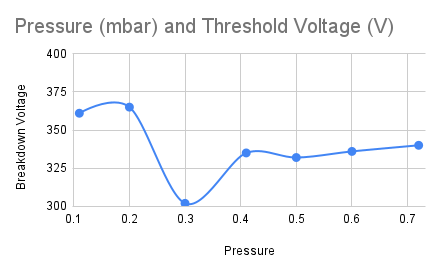
\includegraphics[width=10 cm]{plasma1.png}
\end{center}

	
\subsection{Argon when the Ring is Anode}
\begin{center}
\begin{tabular}{|c|c|c|c|c|}
	\hline
	\multicolumn{1}{|l|}{Base Pressure (mbar)} & \multicolumn{1}{l|}{Pressure (mbar)} & \multicolumn{1}{l|}{Threshold Voltage (V)} & \multicolumn{1}{l|}{Current (mA)} & \multicolumn{1}{l|}{Pressure} \\ \hline
	0.035                                      & 0.12                                 & 322                                        & 31                                & 0.1                           \\ \hline
	0.028                                      & 0.2                                  & 300                                        & 26                                & 0.2                           \\ \hline
	0.027                                      & 0.3                                  & 275                                        & 11                                & 0.3                           \\ \hline
	0.027                                      & 0.41                                 & 265                                        & 8                                 & 0.4                           \\ \hline
	0.027                                      & 0.5                                  & 264                                        & 8                                 & 0.5                           \\ \hline
	0.027                                      & 0.6                                  & 268                                        & 10                                & 0.6                           \\ \hline
	0.026                                      & 0.71                                 & 272                                        & 12                                & 0.72                          \\ \hline
\end{tabular}
	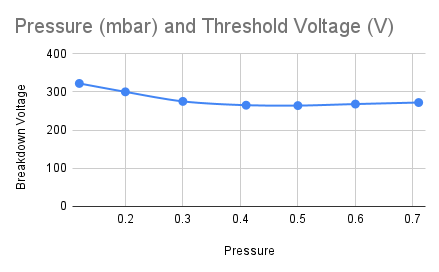
\includegraphics[width=10 cm]{plasma2.png}
\end{center}
\textit{ We are not increasing the Voltage by 25 V and analysing this time considering high current, which may damage the apparatus}
	
\subsection{Nitrogen where the Ring is Cathode}
\begin{center}
	\begin{tabular}{|c|c|c|c|c|c|c|}
		\hline
		Base Pressure (mbar) & Pressure (mbar) & Threshold Voltage (V) & Current (mA) & Pressure & Voltage + 25 & Current (mA) \\ \hline
		0.036                & 0.12            & 555                   & 3            & 0.1      & 570          & 3            \\ \hline
		0.029                & 0.2             & 525                   & 4            & 0.2      & 540          & 3            \\ \hline
		0.02                 & 0.3             & 498                   & 4            & 0.3      & 513          & 4            \\ \hline
		0.029                & 0.4             & 477                   & 5            & 0.4      & 495          & 5            \\ \hline
		0.029                & 0.5             & 478                   & 6            & 0.51     & 493          & 6            \\ \hline
		0.028                & 0.61            & 472                   & 6            & 0.61     & 487          & 7            \\ \hline
		0.029                & 0.71            & 476                   & 7            & 0.72     & 491          & 7            \\ \hline
	\end{tabular}
	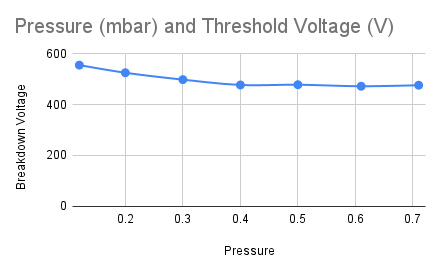
\includegraphics[width=10 cm]{plasma3.png}
\end{center}



\subsection{Nitrogen when the Ring is Anode}
\begin{center}
	\begin{tabular}{|c|c|c|c|c|}
		\hline
		Base Pressure (mbar) & Pressure (mbar) & Threshold Voltage (V) & Current (mA) & Pressure \\ \hline
		0.028                & 0.2             & 510                   & 84           & 0.2      \\ \hline
		0.03                 & 0.3             & 468                   & 71           & 0.3      \\ \hline
		0.029                & 0.4             & 394                   & 32           & 0.4      \\ \hline
		0.029                & 0.5             & 382                   & 24           & 0.51     \\ \hline
		0.029                & 0.61            & 378                   & 21           & 0.61     \\ \hline
		0.029                & 0.71            & 378                   & 18           & 0.72     \\ \hline
	\end{tabular}\\
	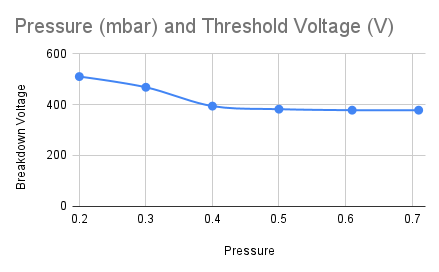
\includegraphics[width=10 cm]{plasma4.png}
\end{center}


*\textit{ We are not increasing the Voltage by 25 V and analysing this time considering high current, which may damage the apparatus}\\
The discrepancies in the shape of the Paschen curve may arise due to the fact that the Paschen curve is derived considering parallel plate condition while we have taken a ring and pipe structure.
\section{Analysis}
\subsection*{Trying to find the Townsend coefficient}
We have the Paschen curve formula
\[V = \frac{Bpd}{ln\bigg(\frac{Apd}{ln(1+\gamma^{-1})}\bigg)}\]
Minimizing, we get
\[V_{min}=2.71828\frac{B}{A}ln(\gamma^{-1}+1)\]
We have the data for B and A as (In $(Pa .m)^{-1}$)\\
\begin{center}
	\begin{tabular}{|c|c|c|}
		\hline
		Gas & A & B \\
		\hline
		$N_2$ & 13 & 413 \\
		\hline
		Ar & 16 & 240 \\
		\hline
	\end{tabular}
\end{center}
Now we make a Hypothesis to find out an approximate Townsend coefficient.\\
\textbf{Approximation:} The minimum V obtained in the experiment can be taken as the minimum V for the Paschen curve.
So if we rewrite the expression for $V_min$ as
\[\frac{1}{\gamma}=exp\bigg(\frac{V_{min}.A}{2.71828.B} \bigg)-1\]
We get approximate Townsend coefficient as
\begin{center}
	\begin{tabular}{|c|c|c|}
		\hline
		Gas & $\gamma$ when ring is anode & $\gamma$ when ring is cathode \\
		\hline
		$N_2$ & 0.07  & 0.09  \\
		\hline
		Ar & 0.06 & 0.052 \\
		\hline
	\end{tabular}
\end{center}

\chapter{Optical Emission Spectroscopy(OES)}
\section{Observations:}
\subsection{Variation of Voltage for the Same Pressure}
\subsubsection{Nitrogen}
\begin{center}
	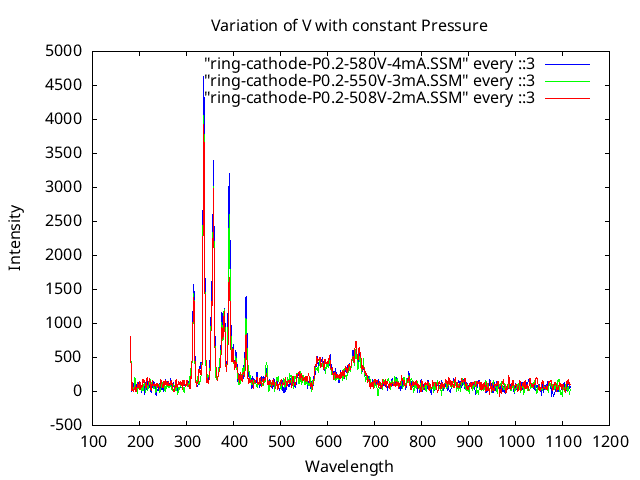
\includegraphics[width=10cm]{VvsP0.2N.png}
\end{center}
\subsubsection{Argon}
\begin{center}
	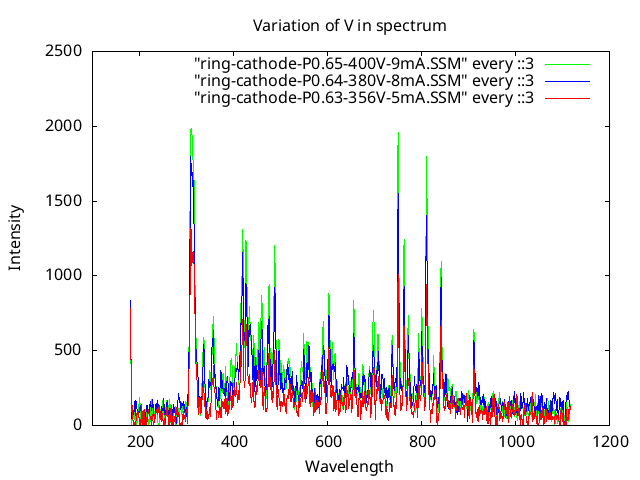
\includegraphics[width=9cm]{P0.64VAr.png}
	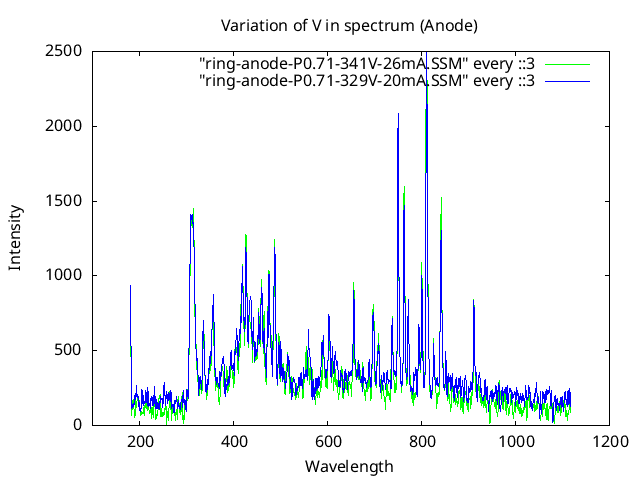
\includegraphics[width=9 cm]{P0.71V(anode)Ar.png}
\end{center}
\subsection{Variation of Pressure for the Same Voltage}
\subsubsection{Nitrogen}
\begin{center}
	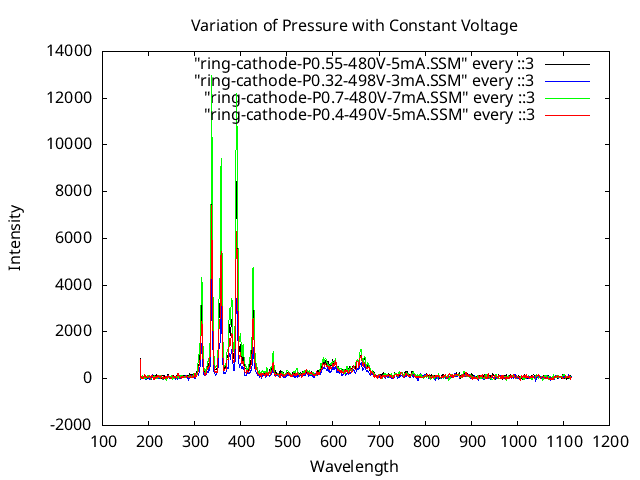
\includegraphics[width=10cm]{PvsV480N.png}
\end{center}
\subsubsection{Argon}
\begin{center}
	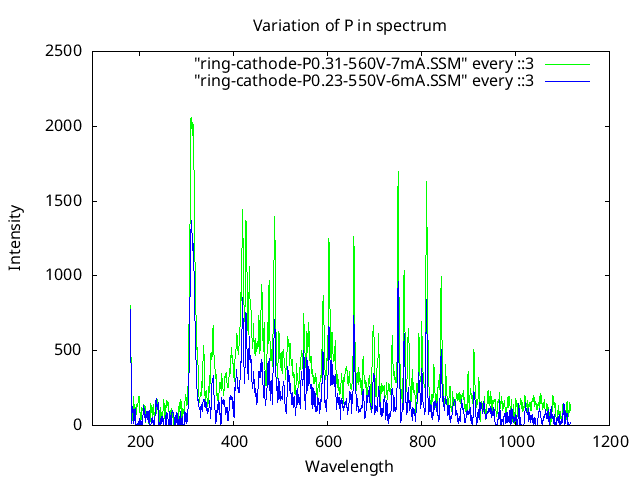
\includegraphics[width=9cm]{PV555Ar.png}
	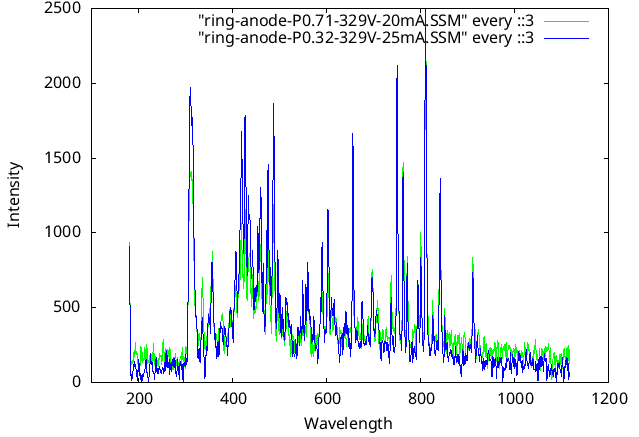
\includegraphics[width=9 cm]{PV329(anode)Armod.png}
\end{center}

\subsection{Nitrogen with ring as anode }
\begin{center}
	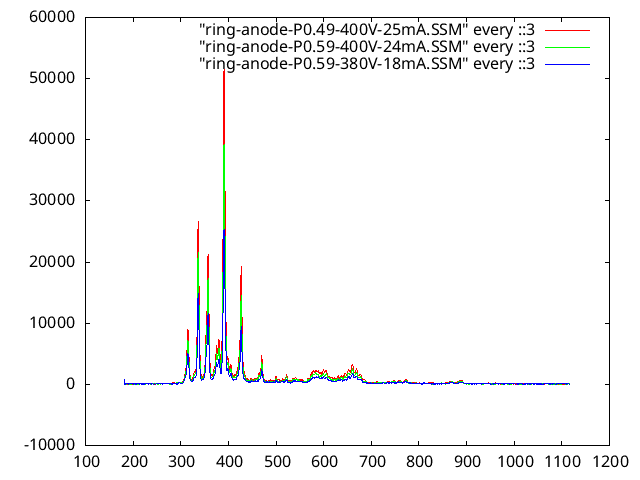
\includegraphics[width=10cm]{nitrogen_ring_anode.png}
\end{center}

\section{Analysis of the Above Graphs}
\subsubsection{Finding the electron temperature}
We find the electron temperature by using the formula
\[ln\bigg(\frac{\lambda_iI_i}{p_i}\bigg)=\frac{E_k}{kT}+C\]
In Nitrogen as we vary the voltage, we get the electron temperatures as \\
\begin{center}
	\begin{tabular}{|c|c|}
		\hline
		Voltage &  Te(eV) \\
		\hline
		508 & 0.101 \\
		\hline
		550 & 0.115 \\
		\hline
		580 & 0.287 \\
		\hline
	\end{tabular}
\end{center}
As we vary the pressure, we get the electron temperatures as 
\begin{center}
	\begin{tabular}{|c|c|}
		\hline
		Voltage &  Te(eV) \\
		\hline
		0.55 & 0.15 \\
		\hline
		0.32 & 0.166 \\
		\hline
		0.7 & 0.89 \\
		\hline
		0.4&0.215\\
		\hline
	\end{tabular}
\end{center}
\section*{Inferences and results:}
In case 1, we see that the electron temperature increases as we increase voltage, which is expected as we are supplying more energy for the breaking down of electrons.\\
In case 2, we see that the electron temperature decreases and increases as we increase pressure, following the Paschen law.\\
If we shift gas, to a more inert Argon, electron temperature increases as we now need some more energy to ionize the gas. Ar comes around the order of 0.5 eV.
\end{document}